%!TEX root = ../report.tex

\begin{document}

    \chapter{Design Details}
    
        \begin{table}[]
    	\begin{center}
    		\begin{tabular}{| l | l | p{3cm} |}
    			\hline
    			Layer (type)       & Output Shape            & Param \#  \\ \hline
    			Conv2d-1           & {[}-1, 64, 240, 320{]}  & 1,792     \\ \hline
    			ReLU-2             & {[}-1, 64, 240, 320{]}  & 0         \\ \hline
    			BatchNorm2d-3      & {[}-1, 64, 240, 320{]}  & 128       \\ \hline
    			Conv2d-4           & {[}-1, 64, 240, 320{]}  & 36,928    \\ \hline
    			ReLU-5             & {[}-1, 64, 240, 320{]}  & 0         \\ \hline
    			BatchNorm2d-6      & {[}-1, 64, 240, 320{]}  & 128       \\ \hline
    			MaxPool2d-7        & {[}-1, 64, 120, 160{]}  & 0         \\ \hline
    			Conv2d-8           & {[}-1, 128, 120, 160{]} & 73,856    \\ \hline
    			ReLU-9             & {[}-1, 128, 120, 160{]} & 0         \\ \hline
    			BatchNorm2d-10     & {[}-1, 128, 120, 160{]} & 256       \\ \hline
    			Conv2d-11          & {[}-1, 128, 120, 160{]} & 147,584   \\ \hline
    			ReLU-12            & {[}-1, 128, 120, 160{]} & 0         \\ \hline
    			BatchNorm2d-13     & {[}-1, 128, 120, 160{]} & 256       \\ \hline
    			MaxPool2d-14       & {[}-1, 128, 60, 80{]}   & 0         \\ \hline
    			Conv2d-15          & {[}-1, 256, 60, 80{]}   & 295,168   \\ \hline
    			ReLU-16            & {[}-1, 256, 60, 80{]}   & 0         \\ \hline
    			BatchNorm2d-17     & {[}-1, 256, 60, 80{]}   & 512       \\ \hline
    			Conv2d-18          & {[}-1, 256, 60, 80{]}   & 590,080   \\ \hline
    			ReLU-19            & {[}-1, 256, 60, 80{]}   & 0         \\ \hline
    			BatchNorm2d-20     & {[}-1, 256, 60, 80{]}   & 512       \\ \hline
    			MaxPool2d-21       & {[}-1, 256, 30, 40{]}   & 0         \\ \hline
    			Conv2d-22          & {[}-1, 512, 30, 40{]}   & 1,180,160 \\ \hline
    			ReLU-23            & {[}-1, 512, 30, 40{]}   & 0         \\ \hline
    			BatchNorm2d-24     & {[}-1, 512, 30, 40{]}   & 1,024     \\ \hline
    			Conv2d-25          & {[}-1, 512, 30, 40{]}   & 2,359,808 \\ \hline
    			ReLU-26            & {[}-1, 512, 30, 40{]}   & 0         \\ \hline
    			BatchNorm2d-27     & {[}-1, 512, 30, 40{]}   & 1,024     \\ \hline
    			MaxPool2d-28       & {[}-1, 512, 15, 20{]}   & 0         \\ \hline
    			Conv2d-29          & {[}-1, 1024, 15, 20{]}  & 4,719,616 \\ \hline
    			ReLU-30            & {[}-1, 1024, 15, 20{]}  & 0         \\ \hline
    			BatchNorm2d-31     & {[}-1, 1024, 15, 20{]}  & 2,048     \\ \hline
    			Conv2d-32          & {[}-1, 1024, 15, 20{]}  & 9,438,208 \\ \hline
    			ReLU-33            & {[}-1, 1024, 15, 20{]}  & 0         \\ \hline
    			BatchNorm2d-34     & {[}-1, 1024, 15, 20{]}  & 2,048     \\ \hline
    			ConvTranspose2d-35 & {[}-1, 512, 30, 40{]}   & 4,719,104 \\ \hline
    			Conv2d-36          & {[}-1, 512, 30, 40{]}   & 4,719,104 \\ \hline
    			ReLU-37            & {[}-1, 512, 30, 40{]}   & 0         \\ \hline
    			BatchNorm2d-38     & {[}-1, 512, 30, 40{]}   & 1,024     \\ \hline
    			Conv2d-39          & {[}-1, 512, 30, 40{]}   & 2,359,808 \\ \hline
    			ReLU-40            & {[}-1, 512, 30, 40{]}   & 0         \\ \hline
    			BatchNorm2d-41     & {[}-1, 512, 30, 40{]}   & 1,024     \\ \hline

    		\end{tabular}
    		\caption{Unet vanilla model architecture}
    		\label{table:unet_vanilla_model_1}
    	\end{center}
    \end{table}
    
    \begin{table}[]
    	\begin{center}
    		\begin{tabular}{| l | l | p{3cm} |}
    			\hline
    			ConvTranspose2d-42 & {[}-1, 256, 60, 80{]}   & 1,179,904 \\ \hline
				Conv2d-43          & {[}-1, 256, 60, 80{]}   & 1,179,904 \\ \hline
				ReLU-44            & {[}-1, 256, 60, 80{]}   & 0         \\ \hline
				BatchNorm2d-45     & {[}-1, 256, 60, 80{]}   & 512       \\ \hline
				Conv2d-46          & {[}-1, 256, 60, 80{]}   & 590,080   \\ \hline
				ReLU-47            & {[}-1, 256, 60, 80{]}   & 0         \\ \hline
				BatchNorm2d-48     & {[}-1, 256, 60, 80{]}   & 512       \\ \hline
				ConvTranspose2d-49 & {[}-1, 128, 120, 160{]} & 295,040   \\ \hline
				Conv2d-50          & {[}-1, 128, 120, 160{]} & 295,040   \\ \hline
    			ReLU-51            & {[}-1, 128, 120, 160{]} & 0         \\ \hline
    			BatchNorm2d-52     & {[}-1, 128, 120, 160{]} & 256       \\ \hline
    			Conv2d-53          & {[}-1, 128, 120, 160{]} & 147,584   \\ \hline
    			ReLU-54            & {[}-1, 128, 120, 160{]} & 0         \\ \hline
    			BatchNorm2d-55     & {[}-1, 128, 120, 160{]} & 256       \\ \hline
    			ConvTranspose2d-56 & {[}-1, 64, 240, 320{]}  & 73,792    \\ \hline
    			Conv2d-57          & {[}-1, 64, 240, 320{]}  & 73,792    \\ \hline
    			ReLU-58            & {[}-1, 64, 240, 320{]}  & 0         \\ \hline
    			BatchNorm2d-59     & {[}-1, 64, 240, 320{]}  & 128       \\ \hline
    			Conv2d-60          & {[}-1, 64, 240, 320{]}  & 36,928    \\ \hline
    			ReLU-61            & {[}-1, 64, 240, 320{]}  & 0         \\ \hline
    			BatchNorm2d-62     & {[}-1, 64, 240, 320{]}  & 128       \\ \hline
    			Conv2d-63          & {[}-1, 41, 240, 320{]}  & 23,657    \\ \hline
    		\end{tabular}
    		\caption{Unet vanilla model architecture}
    		\label{table:unet_vanilla_model_2}
    	\end{center}
    \end{table}

    \chapter{Parameters}
        \begin{table}[h]
    	\begin{center}
    		\begin{tabular}{ | l | p{14cm} |}
    			\hline
    			
    			\cellcolor{purple!30}Id & \cellcolor{purple!30}Classes \\ \hline
    			
    			1 & Wall, Shower Walls, Closet Wall, Shower Wall, Pantry Wall, Closet Walls, Bath Walls, Pantry Walls, Door Wall, \\ \hline
    			2 & Floor, Shower Floor, Closet Floor, \\ \hline
    			3 & Cabinet, Kitchen Cabinet, Kitchen Cabinets, File Cabinet, Bathroom Vanity, Cabinets, Bathroom Cabinet, Cabinet Doors, Open Kitchen Cabinet, File Cabinets, Trash Cabinet, Media Center, \\ \hline
    			4 & Bed, Mattress, Loft Bed, Sofa Bed, Air Mattress, \\ \hline
    			5 & Chair, Office Chair, Armchair, Sofa Chair, Stack Of Chairs, Folded Chair, Folded Chairs, Massage Chair, Recliner Chair, Rocking Chair, Stack Of Folded Chairs, \\ \hline
    			6 & Couch, Sofa, \\ \hline
    			7 & Table, Coffee Table, End Table, Dining Table, Folded Table, Round Table, Side Table, Air Hockey Table, \\ \hline
    			8 & Door, Doorframe, Doors, Bathroom Stall Door, Closet Doors, Closet Door, Shower Door, Mirror Doors, Cabinet Door, Glass Doors, Sliding Door, Closet Doorframe, \\ \hline
    			9 & Window, \\ \hline
    			10 & Bookshelf, Bookshelves, \\ \hline
    			11 & Picture, Poster, Painting, Pictures, \\ \hline
    			12 & Kitchen Counter, Counter, Bathroom Counter, \\ \hline
    			13 & Blinds, \\ \hline
    			14 & Desk, \\ \hline
    			15 & Shelf, Organizer Shelf, Pantry Shelf, Closet Shelf, \\ \hline
    			16 & Curtain, Curtains, \\ \hline
    			17 & Dresser, \\ \hline
    			18 & Pillow, Pillows, Couch Cushions, Cushion, \\ \hline
    			19 & Mirror, \\ \hline
    			20 & Mat, Yoga Mat, \\ \hline
    			21 & Clothes, Clothing, Cloth, Sock, Kitchen Apron, Costume, Socks, \\ \hline
    			22 & Ceiling, Closet Ceiling, \\ \hline
    			23 & Books, Book, Music Book, \\ \hline
    			24 & Refrigerator, Mini Fridge, Cooler, \\ \hline
    			25 & Tv, \\ \hline
    			26 & Paper, Papers, \\ \hline
    			27 & Towel, Towels, Hand Towel, \\ \hline
    			28 & Shower Curtain, \\ \hline
    			29 & Box, Boxes, Mailboxes, Mailbox, Storage Box, Pizza Box, Boxes Of Paper, Jewelry Box, Cat Litter Box, Covered Box, Pizza Boxes, \\ \hline
    			30 & Whiteboard, \\ \hline
    			31 & Person, Legs, \\ \hline
    			32 & Nightstand, \\ \hline
    			33 & Toilet, Urinal, \\ \hline
    			34 & Sink, \\ \hline
    			35 & Lamp, Lamp Base, Desk Lamp, Wall Lamp, Table Lamp, Ceiling Lamp, Night Lamp, \\ \hline
    			36 & Bathtub, \\ \hline
    			37 & Bag, Paper Bag, Messenger Bag, Ikea Bag, Duffel Bag, Bag Of Coffee Beans, Grocery Bag, Golf Bag, Garbage Bag, Coffee Bean Bag, Trash Bag, Cosmetic Bag, Shopping Bag, Food Bag, \\ \hline
    			
    			\hline
    		\end{tabular}
    		\caption{Classes and ids of the Scannet dataset}
    		\label{table:Classes in scannet_1}
    		
    	\end{center}
    \end{table}
    
    \begin{table}
    	\begin{center}
    		\begin{tabular}{ | l | p{14cm} |}
    			\hline
    			
    			\cellcolor{purple!30}Id & \cellcolor{purple!30}Classes \\ \hline
    			38 & Board, Stove, Light, Bathroom Stall, Bar, Light Switch, Ceiling Light, Range Hood, Blackboard, Rail, Bulletin Board, Ledge, Shower, Windowsill, Dishwasher, Stair Rail, Stairs, Handicap Bar, Column, Oven, Pillar, Structure, Shower Head, Projector Screen, Staircase, Fireplace, Breakfast Bar, Hand Rail, Water Fountain, Kitchen Island, Pipes, Shower Control Valve, Handrail, Step, Dart Board, Grab Bar, Railing, Stair, Soap Bar, Studio Light, Shower Doors, Boards, Frame, Garage Door, Platform, Elevator, Wood Beam, Banister, Curtain Rod, Chandelier, Stovetop, Glass, \\ \hline
    			39 & Trash Can, Radiator, Recycling Bin, Ottoman, Bench, Tv Stand, Wardrobe Closet, Trash Bin, Seat, Closet, Ladder, Piano, Water Cooler, Stand, Washing Machine, Rack, Washing Machines, Wardrobe Cabinet, Clothes Dryer, Ironing Board, Keyboard Piano, Music Stand, Furniture, Crate, Clothes Dryers, Drawer, Footrest, Piano Bench, Foosball Table, Footstool, Compost Bin, Tripod, Treadmill, Chest, Folded Ladder, Drying Rack, Pool Table, Heater, Toolbox, Beanbag Chair, Dollhouse, Ping Pong Table, Clothing Rack, Podium, Luggage Stand, Rack Stand, Futon, Book Rack, Seating, Workbench, Easel, Luggage Rack, Headboard, Display Rack, Crib, Bedframe, Closet Wardrobe, Wardrobe, Bunk Bed, Magazine Rack, Furnace, Stepladder, Baby Changing Station, Flower Stand, Display, \\ \hline
    			\hline
    		\end{tabular}
    		\caption{Classes and ids of the Scannet dataset}
    		\label{table:Classes in scannet_2}
    	\end{center}
    \end{table}
    
    \begin{table}
    	\begin{center}
    		\begin{tabular}{ | l | p{14cm} |}
    			\hline
    			
    			\cellcolor{purple!30}Id & \cellcolor{purple!30}Classes \\ \hline
    			
    			40 & Object, Monitor, Backpack, Plant, Toilet Paper, Shoes, Keyboard, Bottle, Stool, Computer Tower, Telephone, Cup, Jacket, Microwave, Paper Towel Dispenser, Suitcase, Laptop, Printer, Soap Dispenser, Fan, Tissue Box, Blanket, Copier, Soap Dish, Laundry Hamper, Storage Bin, Coffee Maker, Decoration, Clock, Mouse, Basket, Dumbbell, Bucket, Sign, Speaker, Container, Shower Curtain Rod, Tube, Storage Container, Paper Towel Roll, Ball, Laundry Basket, Cart, Dish Rack, Purse, Bicycle, Tray, Plunger, Paper Cutter, Toilet Paper Dispenser, Bin, Toilet Seat Cover Dispenser, Guitar, Fire Extinguisher, Pipe, Vacuum Cleaner, Plate, Cd Case, Bowl, Closet Rod, Scale, Broom, Hat, Guitar Case, Water Pitcher, Laundry Detergent, Hair Dryer, Divider, Power Outlet, Coffee Kettle, Toaster, Shoe, Alarm Clock, Water Bottle, Case Of Water Bottles, Toaster Oven, Coat Rack, Storage Organizer, Machine, Fire Alarm, Vent, Power Strip, Calendar, Toilet Paper Holder, Potted Plant, Stuffed Animal, Luggage, Headphones, Candle, Projector, Dustpan, Rod, Globe, Step Stool, Vending Machine, Ceiling Fan, Swiffer, Jar, Hamper, Poster Tube, Case, Carpet, Thermostat, Coat, Smoke Detector, Flip Flops, Banner, Clothes Hanger, Whiteboard Eraser, Iron, Instrument Case, Toilet Paper Rolls, Soap, Block, Wall Hanging, Toothbrush, Shirt, Cutting Board, Vase, Exercise Machine, Shorts, Tire, Teddy Bear, Bathrobe, Faucet, Thermos, Rug, Tupperware, Shoe Rack, Beer Bottles, Salt, Dispenser, Remote, Carton, Slippers, Soda Stream, Toilet Brush, Cooking Pot, Stapler, Scanner, Elliptical Machine, Kettle, Metronome, Dumbell, Rice Cooker, Sewing Machine, Flowerpot, Nerf Gun, Binders, Quadcopter, Pitcher, Hanging, Mail, Hoverboard, Water Heater, Spray Bottle, Rope, Plastic Container, Soap Bottle, Sleeping Bag, Frying Pan, Oven Mitt, Pot, Hand Dryer, Shampoo Bottle, Hair Brush, Tennis Racket, Display Case, Boiler, Bananas, Carseat, Helmet, Umbrella, Coffee Box, Envelope, Wet Floor Sign, Controller, Dolly, Shampoo, Paper Tray, Changing Station, Poster Printer, Screen, Crutches, Stack Of Cups, Toilet Flush Button, Trunk, Plastic Bin, Car, Shaving Cream, Shredder, Statue, Hose, Bike Pump, Coatrack, Bear, Humidifier, Toothpaste, Mouthwash Bottle, Poster Cutter, Food Container, Camera, Card, Mug, Cardboard, Flag, Magazine, Exit Sign, Rolled Poster, Wheel, Blackboard Eraser, Organizer, Doll, Laundry Bag, Sponge, Lotion Bottle, Can, Lunch Box, Food Display, Storage Shelf, Sliding Wood Door, Pants, Wood, Bottles, Washcloth, Cups, Exercise Ball, Roomba, Bike Lock, Briefcase, Bath Products, Star, Map, Ipad, Traffic Cone, Toiletry, Canopy, Paper Organizer, Barricade, Cap, Dumbbell Plates, Cooking Pan, Santa, Boat, Kinect, Plastic Storage Bin, Dishwashing Soap Bottle, Xbox Controller, Banana Holder, Ping Pong Paddle, Airplane, Conditioner Bottle, Tea Kettle, Toilet Paper Package, Wall Mounted Coat Rack, Film Light, Chain, Sweater, Kitchen Mixer, Water Softener, Trolley, Loofa, Shower Faucet Handle, Toy Piano, Fish, Electric Panel, Suitcases, Tape, Plates, Alarm, Fire Hose, Toy Dinosaur, Cone, Hatrack, Subwoofer, Fire Sprinkler, Photo, Barrier, Stacks Of Cups, Beachball, Folded Boxes, Contact Lens Solution Bottle, Folder, Mail Trays, Slipper, Sticker, Lotion, Buddha, File Organizer, Paper Towel Rolls, Fuse Box, Knife Block, Cd Cases, Stools, Hand Sanitzer Dispenser, Teapot, Pen Holder, Tray Rack, Wig, Switch, Plastic Containers, Night Light, Notepad, Mail Bin, Elevator Button, Gaming Wheel, Drum Set, Coffee Mug, Baby Mobile, Diaper Bin, Stepstool, Paper Shredder, Dress Rack, Cover, Exercise Bike, Kitchenaid Mixer, Soda Can, Tap, Cable, Binder, Towel Rack, Medal, Telescope, Baseball Cap, Battery Disposal Jar, Mop, Tank, Mail Tray, Centerpiece, Stick, Dryer Sheets, Bycicle, Clip, Postcard, Display Sign, Paper Towel, Boots, Tennis Racket Bag, Clothes Hangers, Starbucks Cup, \\ \hline
    			
    			0 & Other \\ \hline
    			\hline
    			
    			
    		\end{tabular}
    		\caption{Classes and ids of the Scannet dataset}
    		\label{table:Classes in scannet_3}
    	\end{center}
    \end{table}
	
 	\begin{table}
		\begin{center}
			\begin{tabular}{ | l | p{16cm} |}
				\hline
				
				\cellcolor{purple!30}Id & \cellcolor{purple!30}Classes \\ \hline
				0 & Other \\ \hline
				1 & Terrain \\ \hline
				2 & Sky \\ \hline
				3 & Tree \\ \hline
				4 & Vegetation \\ \hline
				5 & Building \\ \hline
				6 & Road \\ \hline
				7 & Guardrail \\ \hline
				8 & Traffic Sign \\ \hline
				9 & Traffic light \\ \hline
				10 & Pole \\ \hline
				11 & Misc \\ \hline
				12 & Truck \\ \hline
				13 & Car \\ \hline
				14 & Van \\ \hline
				\hline
			\end{tabular}
			\caption{Vkitti dataset classes}
			\label{table:Classes in scannet_2}
		\end{center}
	\end{table}
	
	\begin{figure}
		\centering
		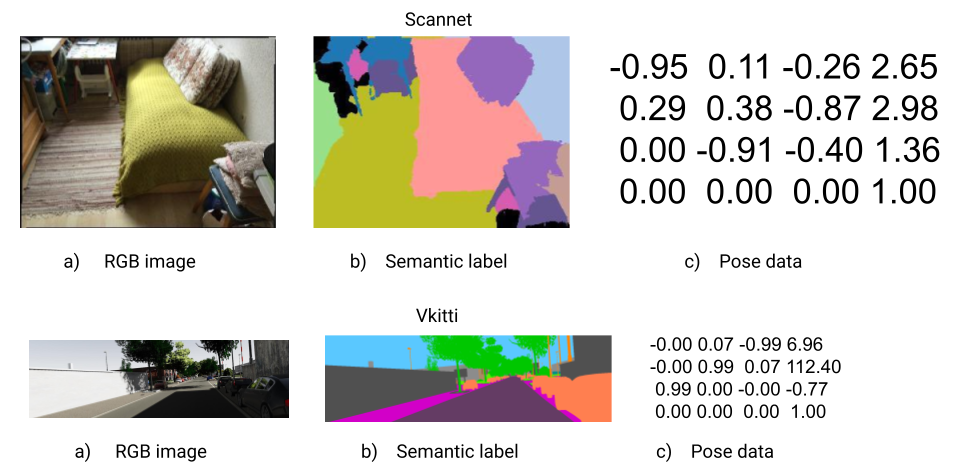
\includegraphics[width=13cm]{images/dataset.png}
		\caption{Scannet and vkitti dataset sample}
		\label{fig:android_result}
	\end{figure}

	\chapter{Training details}
	
	\begin{figure}
		\centering
		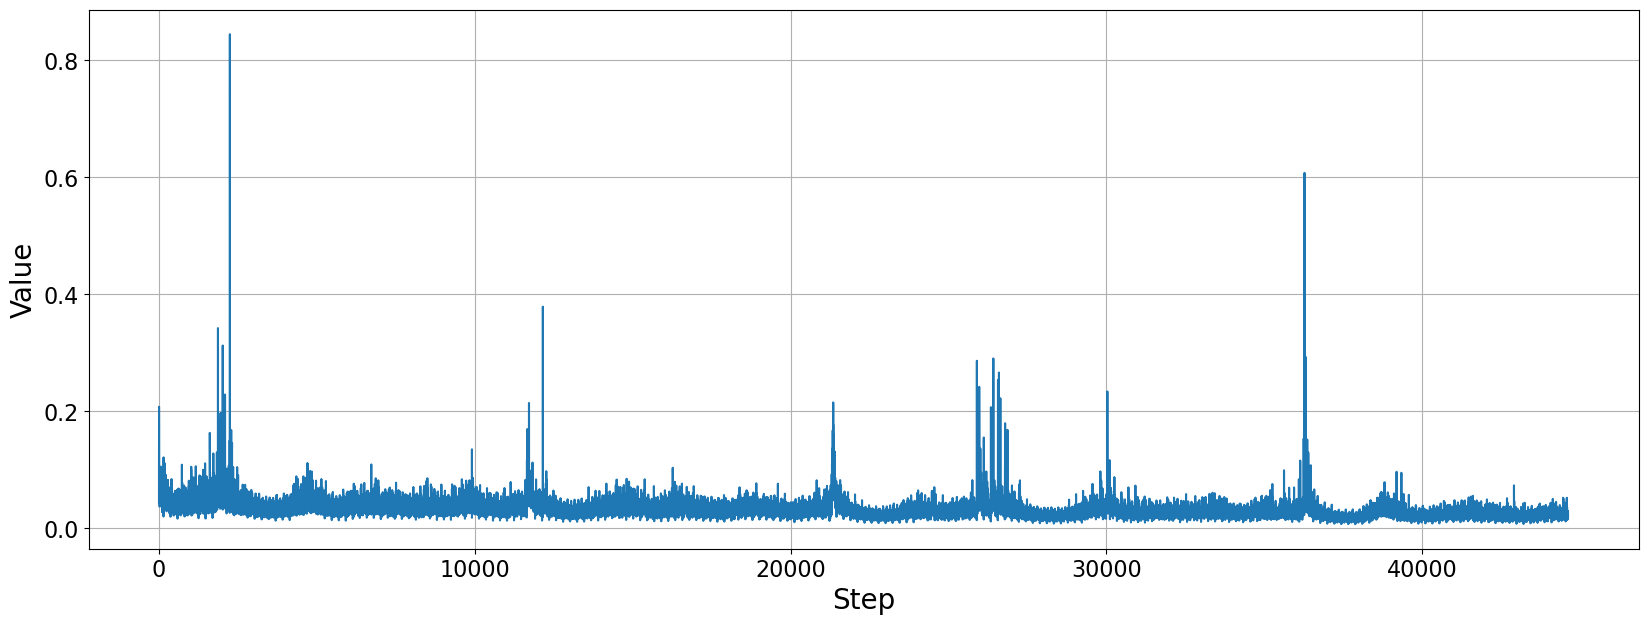
\includegraphics[width=13cm]{images/scannet_step_vanilla_all.png}
		\caption{Scannet step losses for vanilla}
		\label{fig:android_result}
	\end{figure}

	\begin{figure}
		\centering
		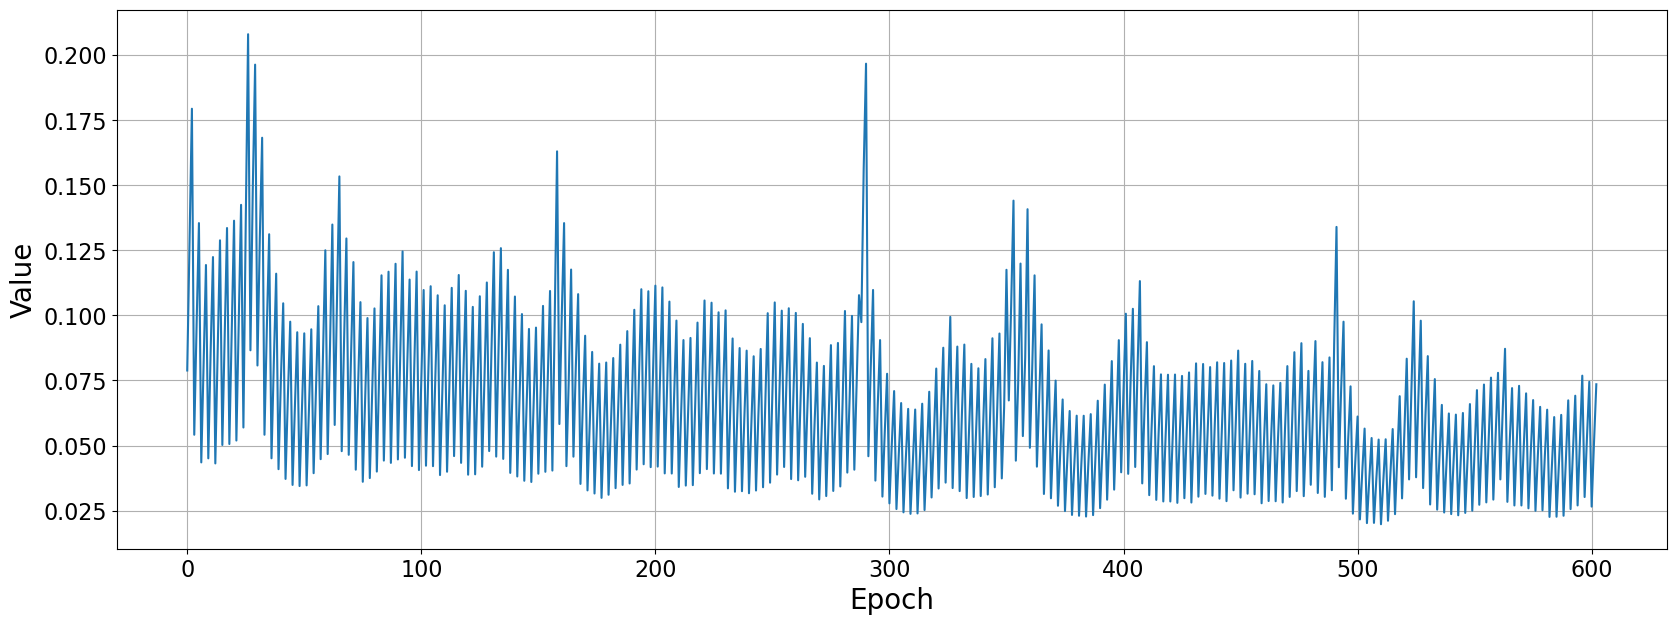
\includegraphics[width=13cm]{images/scannet_epoch_vanilla_all.png}
		\caption{Scannet epoch losses for vanilla}
		\label{fig:android_result}
	\end{figure}

	\begin{figure}
		\centering
		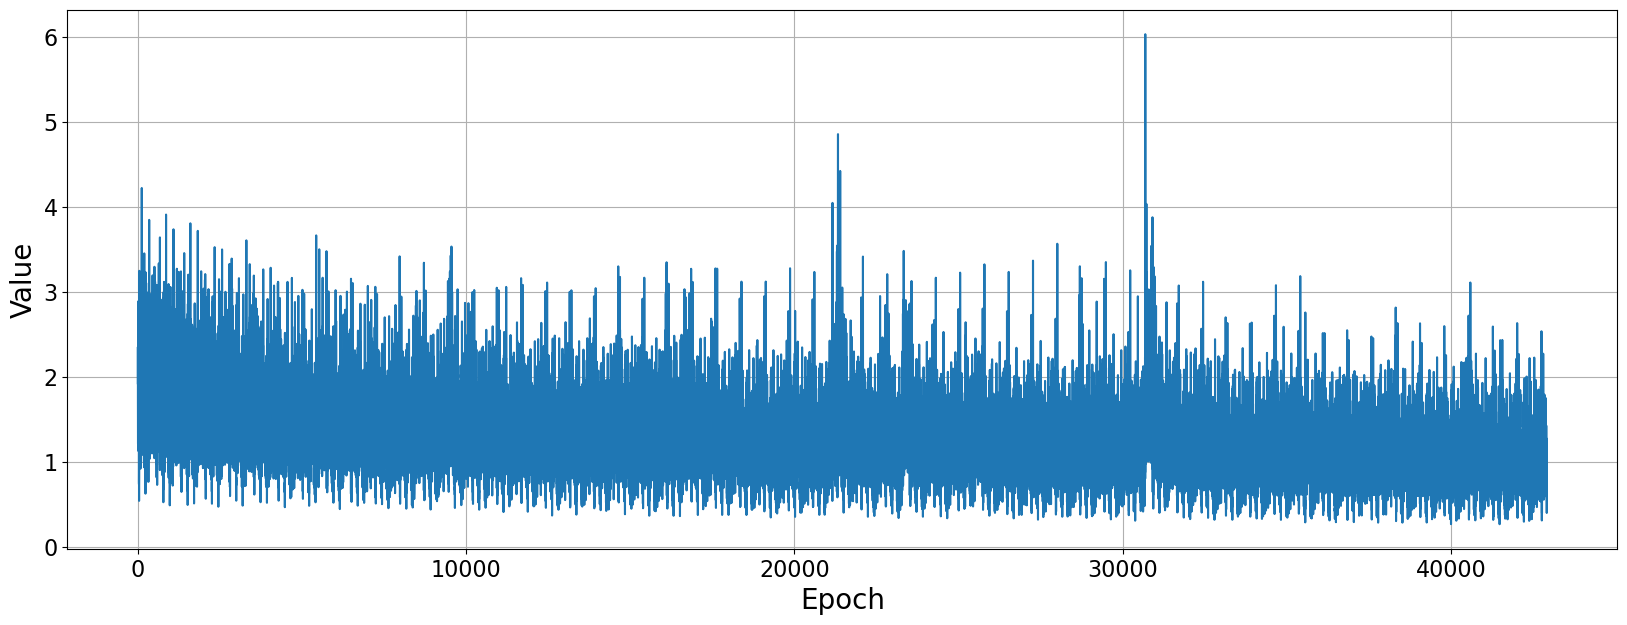
\includegraphics[width=13cm]{images/scannet_gp_step.png}
		\caption{Scannet step losses for GP}
		\label{fig:android_result}
	\end{figure}

	\begin{figure}
		\centering
		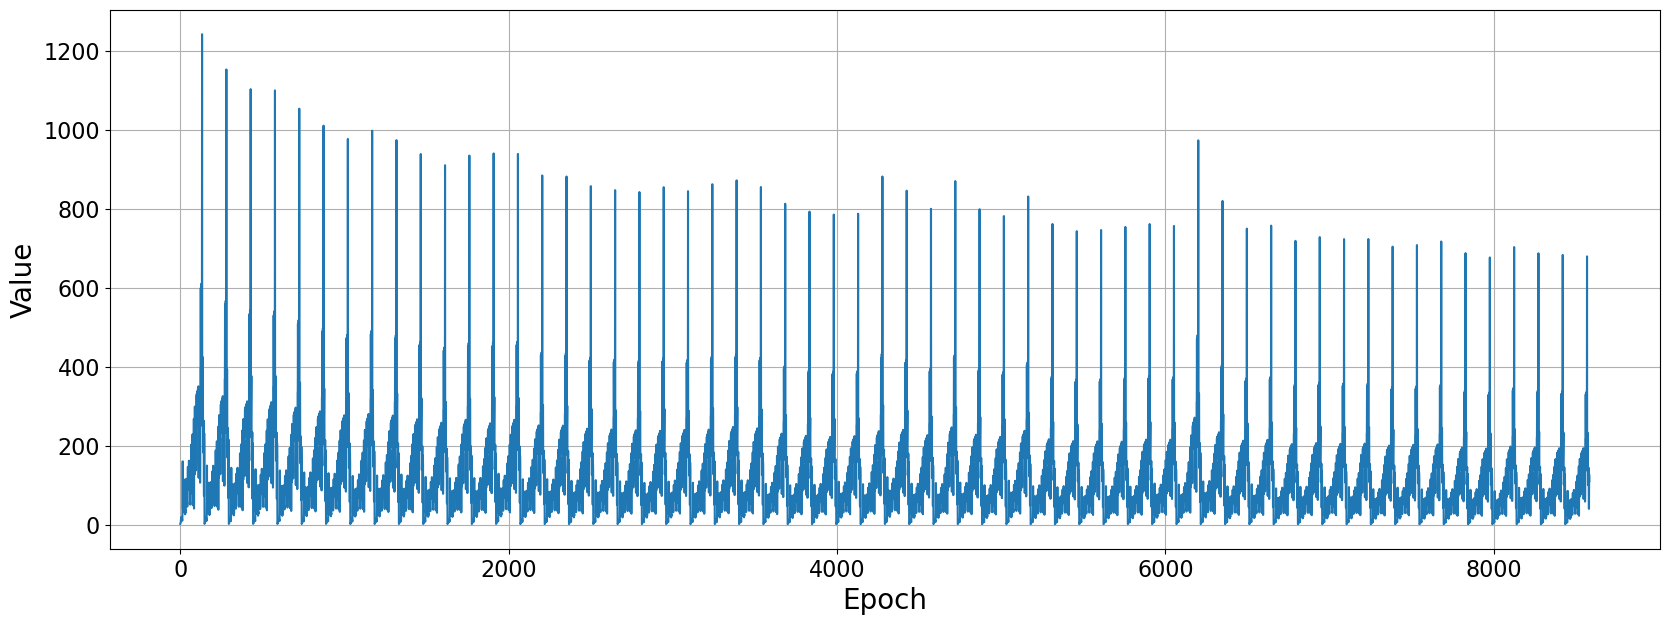
\includegraphics[width=13cm]{images/scannet_gp_epoch_all.png}
		\caption{Scannet epoch losses for GP}
		\label{fig:android_result}
	\end{figure}

	\begin{figure}
		\centering
		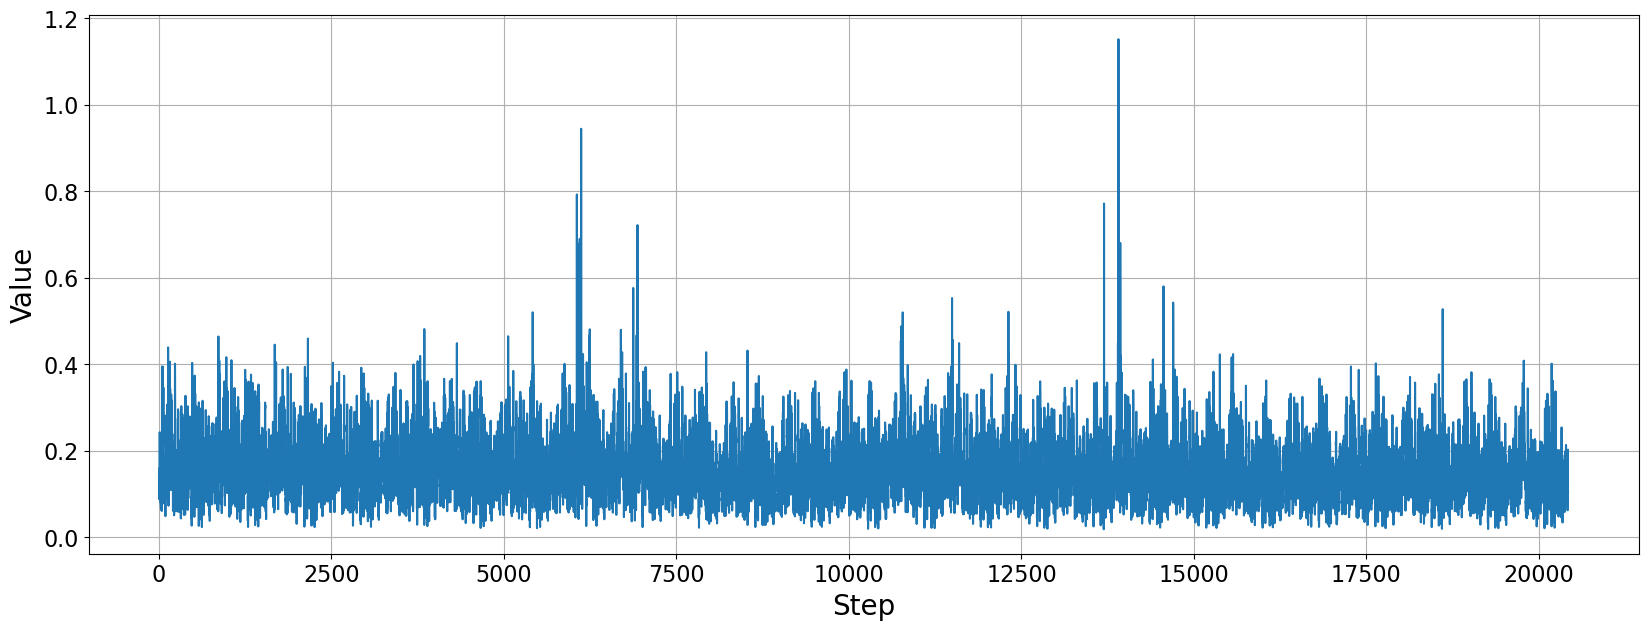
\includegraphics[width=13cm]{images/scannet_step_lstm.png}
		\caption{Scannet step losses for lstm}
		\label{fig:android_result}
	\end{figure}

	\begin{figure}
		\centering
		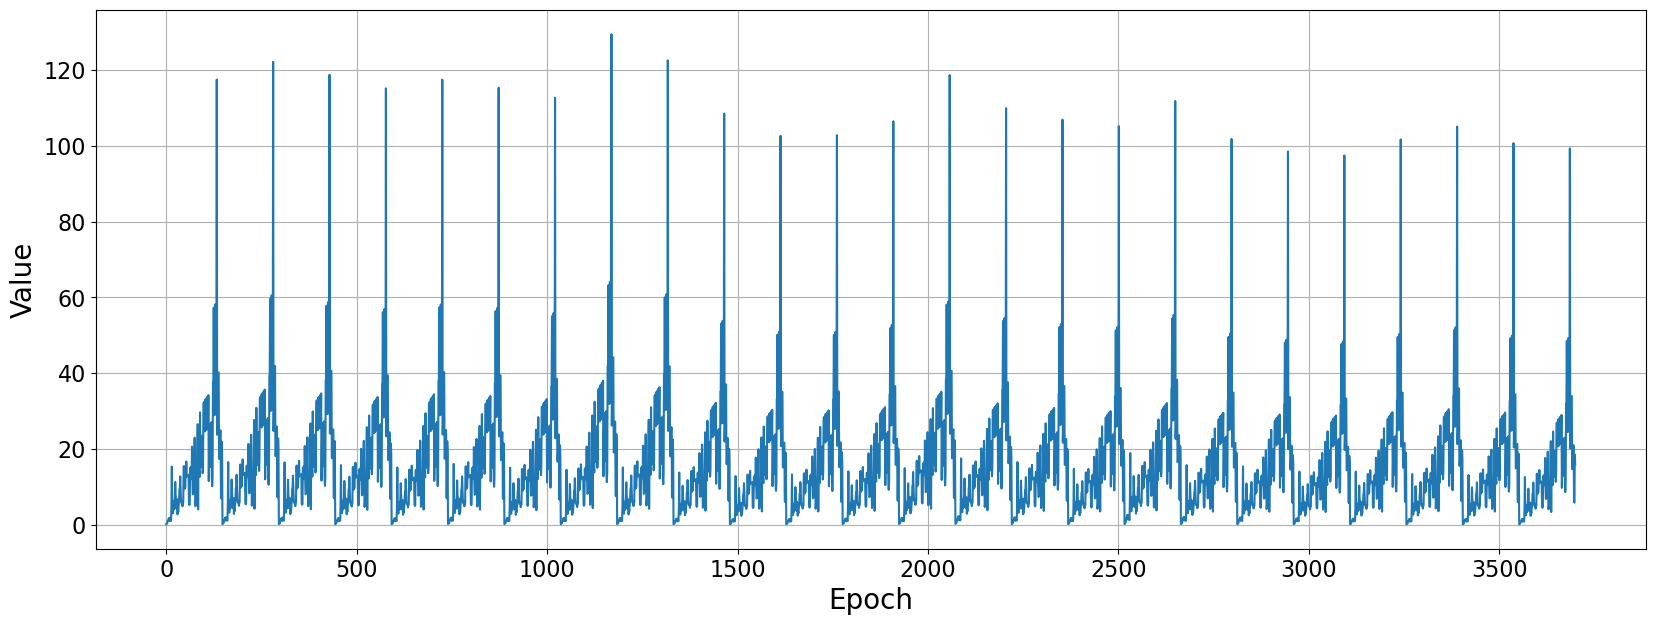
\includegraphics[width=13cm]{images/scannet_lstm_epoch_all.png}
		\caption{Scannet epoch losses for lstm}
		\label{fig:android_result}
	\end{figure}

	\begin{figure}
		\centering
		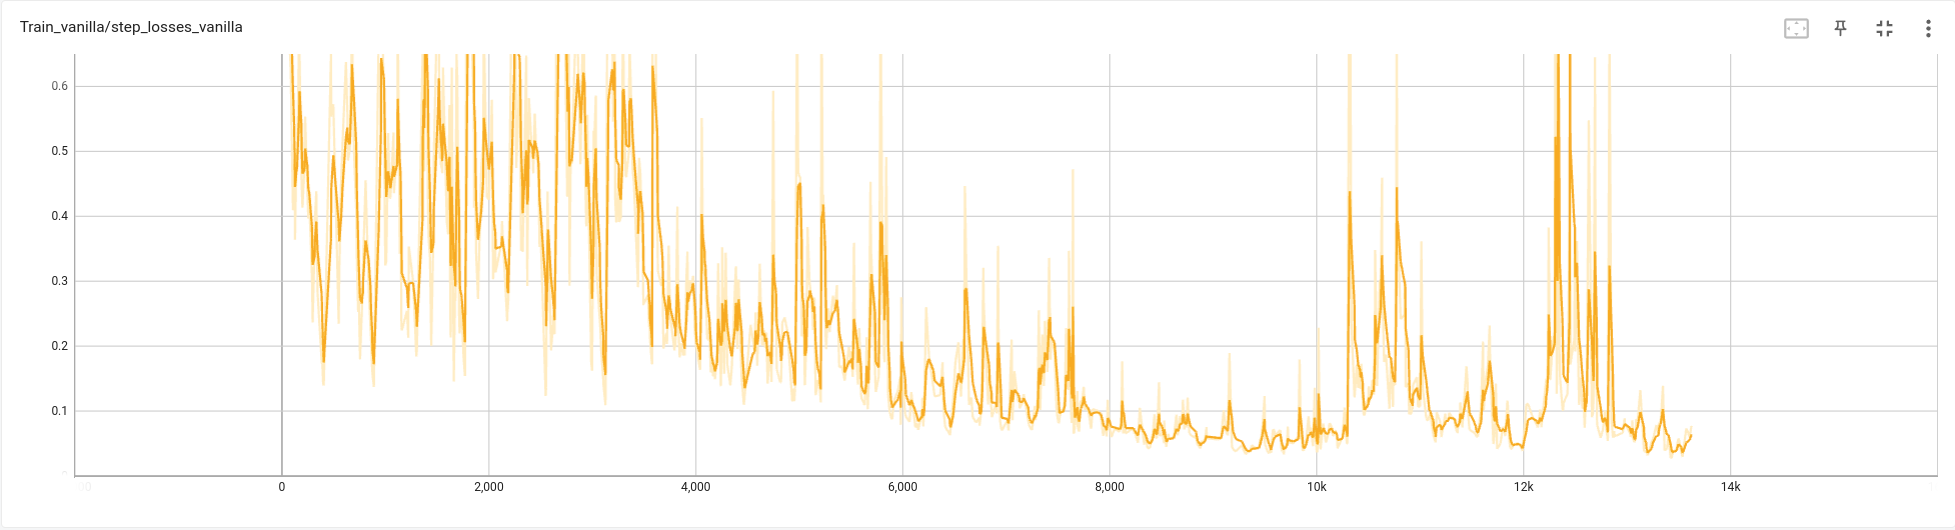
\includegraphics[width=13cm]{images/vanilla_step_loss_vkitti.png}
		\caption{Vkitti step loss vanilla}
		\label{fig:android_result}
	\end{figure}

	\begin{figure}
		\centering
		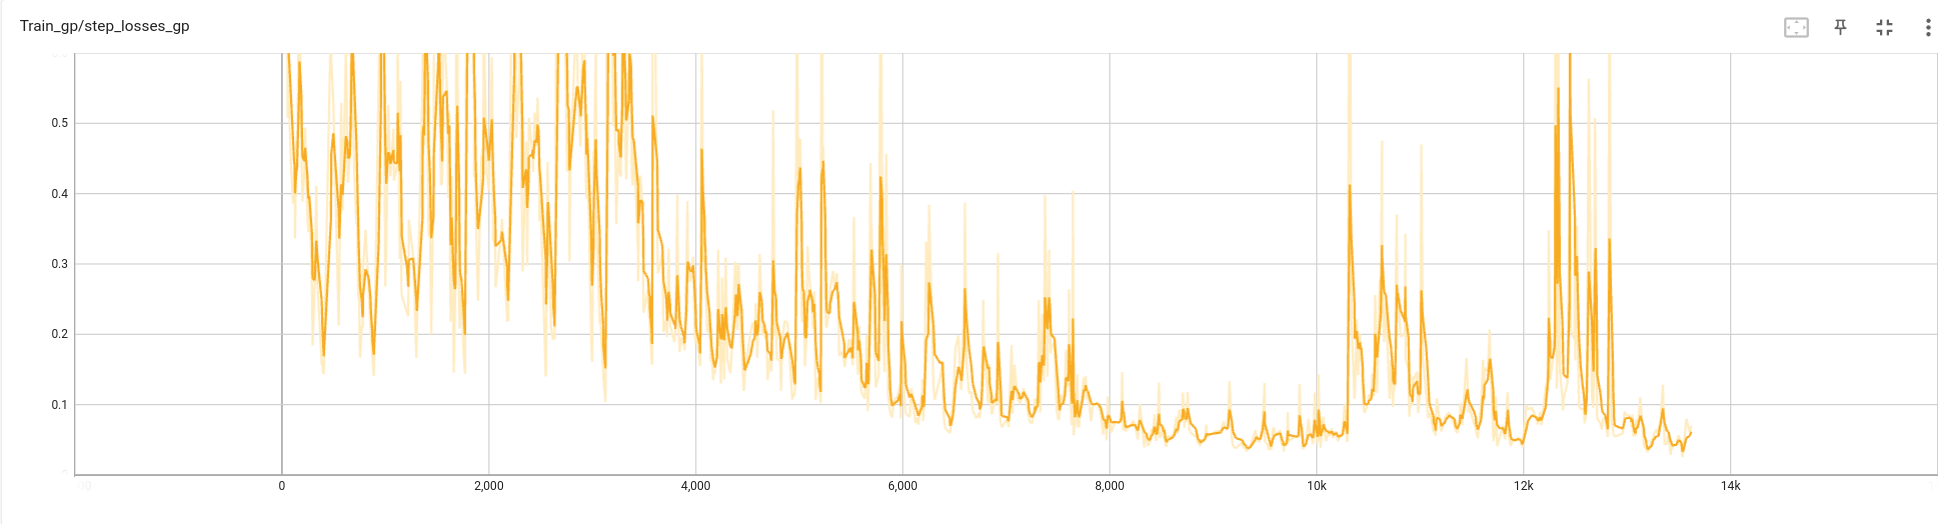
\includegraphics[width=13cm]{images/gp_step_loss_vkitti.png}
		\caption{Vkitti step loss GP}
		\label{fig:android_result}
	\end{figure}

	\begin{figure}
		\centering
		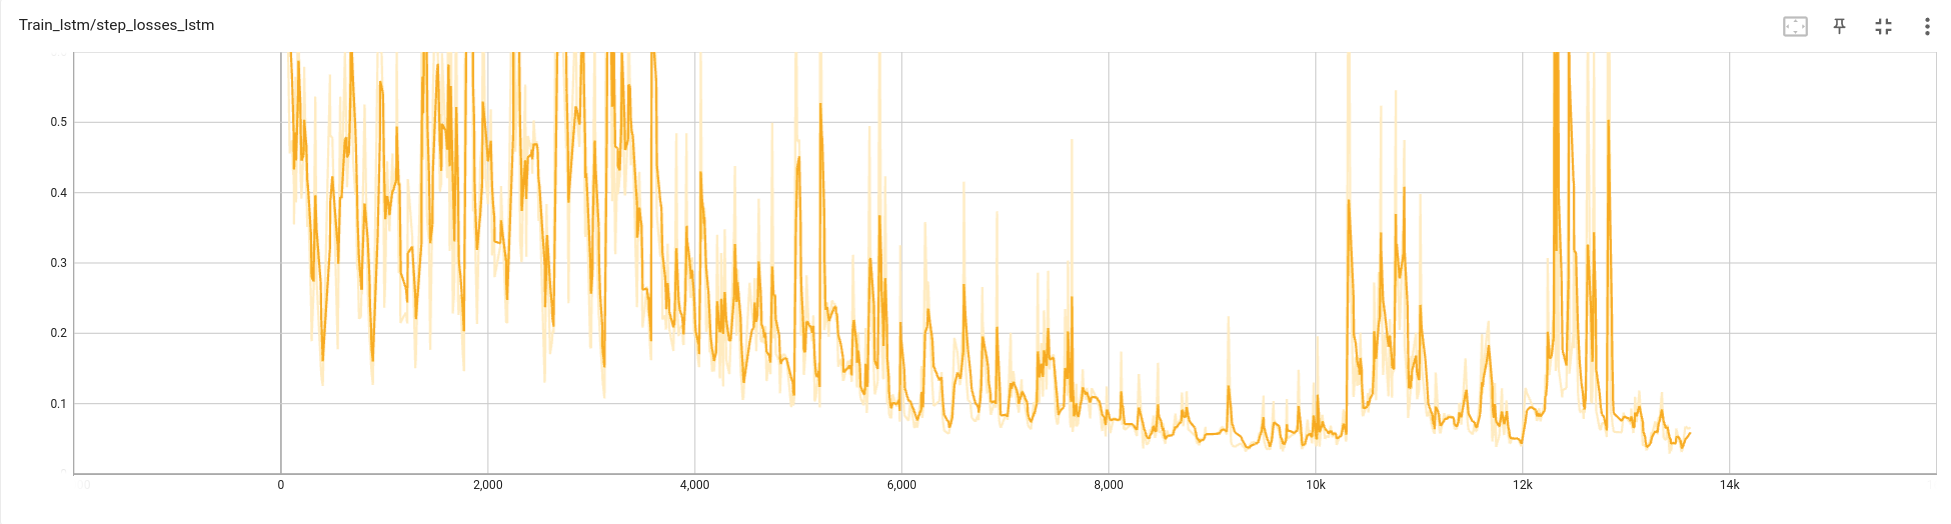
\includegraphics[width=13cm]{images/lstm_step_loss_vkitti.png}
		\caption{Vkitti step loss lstm}
		\label{fig:android_result}
	\end{figure}

	\begin{figure}
		\centering
		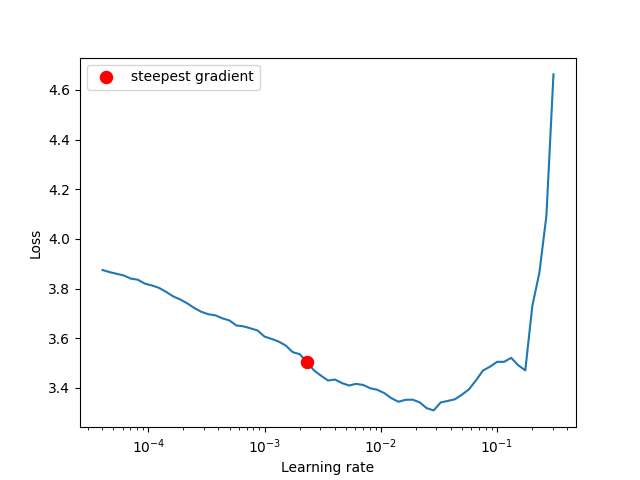
\includegraphics[width=13cm]{images/lr_finder_41.png}
		\caption{Learning rate finder}
		\label{fig:android_result}
	\end{figure}

\end{document}
